\documentclass[avery5371]{flashcards}

\usepackage{amssymb}
\usepackage{amsmath}
\usepackage{datetime}
\usepackage{hyperref}
\usepackage{ragged2e}
\hypersetup{
    colorlinks=false,
}
%\usepackage{transparent}
\usepackage{graphicx}
\graphicspath{{./images/print/}}
\usepackage[export]{adjustbox}
\usepackage{lipsum}
\usepackage{svg}
\usepackage{tikz}
\usepackage[top]{background}
\usepackage{xcolor}
\definecolor{uniscielblue}{RGB}{4,146,191}
\definecolor{uniscielpink}{RGB}{231,33,90}
\definecolor{uniscielgrey}{RGB}{103,104,104}
% Bleu : #0492bf
% Rose : #e7215a
% Gris : #676868

\usepackage{fontspec}
\setsansfont{Eufoniem One}

% --- FONT SIZE --- %
\cardfrontstyle[\footnotesize]{headings}
\cardbackstyle[\footnotesize]{plain}
\usepackage{changepage}
\strictpagecheck
\usetikzlibrary{patterns,calc}

\usepackage{geometry}
%  % --- PAPER SIZE --- %
 \geometry{
    showframe,
    papersize={100truemm,80truemm},
    marginparsep=0cm,
    footskip=0cm,
    hmargin=2mm,
    vmargin=2mm,
 }
\usepackage[
     noinfo,
     cam,
    %  cross,
     width=110truemm,
     height=90truemm,
     center
 ]{crop}
%%%% COMMANDES CUSTOMS %%%%%

\newcommand{\cardfrontfooter}[2]{
    \SetBgContents{\bgimage{0.15}{0.8}{#1}{#2}}   
}

\newcommand{\cardfrontheader}[3]{  
    \begin{tikzpicture}[remember picture, overlay]
        \checkoddpage
        \ifoddpage  
            \node [opacity=1] at ([xshift=0cm, yshift=0cm]current page.center) {
                \includesvg[]{recto-entete}
            };
        \else
            \node [opacity=1] at ([xshift=0cm, yshift=0cm]current page.center) {
                
\includegraphics[max size={\textwidth}{0.5\textheight}, center, keepaspectratio]{qrcode}
            };
        \fi
    \end{tikzpicture}  
    \begin{center}
        \begin{minipage}[c]{0.17\linewidth}
            \vspace{-0.85\baselineskip}
            \includesvg[height=1.1\linewidth]{icons/physique}
        \end{minipage}%
        \hspace{1.5\baselineskip}
        \begin{minipage}[c]{0.74\linewidth}
            \vspace{-\baselineskip}
            \color{uniscielblue}
            \textbf{\textsf{#1}} -- \textsf{\textbf{#2}}\\
            \color{uniscielgrey}
            \rule[1.1mm]{2cm}{0.3mm}\\
            \color{uniscielpink}
            \raggedright
            \textsf{#3}
        \end{minipage}
    \end{center}
}
%%%% IMAGE DE FOND %%%%%
\newcommand{\bgimage}[4]{
    \begin{tikzpicture}[remember picture, overlay]
        \checkoddpage
        \ifoddpage  
            \node [opacity=1] at ([xshift=-5.4cm, yshift=-1.7cm]current page.south) {
                \color{uniscielpink}
                #3
            };
            \node [opacity=1] at ([xshift=0.7cm, yshift=-1.1cm]current page.south) {
                % 
\includegraphics[max size={\textwidth}{0.5\textheight}, center, keepaspectratio]{university_logo}
            };
        \else
            \node [opacity=1] at ([xshift=-1.2cm, yshift=1cm]current page.west) {
                \includesvg[height=0.18\linewidth]{icons/#4}
            };
        \fi
    \end{tikzpicture}
}


% --- CARD SIZE --- %
\renewcommand{\cardpapermode}{portrait}
\renewcommand{\cardrows}{1}
\renewcommand{\cardcolumns}{1}
\setlength{\cardheight}{7.4cm}
\setlength{\cardwidth}{9.5cm}

\newlength{\enoncevspace}
\setlength{\enoncevspace}{0cm}
\newlength{\reponsevspace}
\setlength{\reponsevspace}{0cm}
\setlength{\cardmargin}{1cm}
\setlength{\topoffset}{0mm}
\setlength{\oddoffset}{0mm}
\setlength{\evenoffset}{0mm}

\SetBgScale{1.0}% Select scale factor of logo
\SetBgAngle{0.0}% Select roation of logo
%\SetBgOpacity{0.5}% Select opacity
% \SetBgContents{\bgimage{0.15}{0.8}}% Set tikz picture
%\SetBgPosition{current page.north west}% Select location
% Cadre Rajouté à l'impression



\begin{document}


%%%%%%%%%%%%%%% TEMPLATE STANDARD %%%%%%%%%%%%%%%%

\cardfrontfooter{Niveau de complexité}{physique}
\begin{flashcard}[\cardfrontheader{Matière}{L0}{Thème}]{
%%%%%%%%%%%%%%% ÉNONCÉ %%%%%%%%%%%%%%%%
\vspace{\enoncevspace}
\'Enoncé
\begin{enumerate}
    \item Réponse 1
    \item Réponse 2
    \item Réponse 3
    \item Réponse 4
\end{enumerate}
}
%%%%%%%%%%%%%%% ÉNONCÉ %%%%%%%%%%%%%%%%
\vspace*{\stretch{1}}
%%%%%%%%%%%%%%% RÉPONSE %%%%%%%%%%%%%%%%
\vspace{\reponsevspace}

\begin{tikzpicture}[remember picture, overlay]
    \node [align=left, opacity=1] at ([xshift=-1.75cm, yshift=2.5cm]current page.center) {
                \color{uniscielgrey}
                \textsf{\textit{Réponses}}
            };
    \node [align=left, opacity=1] at ([xshift=1.75cm, yshift=2.5cm]current page.center) {
                \color{uniscielgrey}
                $1:\boxtimes\qquad2:\square\qquad3:\square\qquad4:\square\qquad$\\
                \color{uniscielgrey}
                $5:\square\qquad6:\square\qquad$
            };
\end{tikzpicture}
\lipsum[2]
%%%%%%%%%%%%%%% RÉPONSE %%%%%%%%%%%%%%%%
\vspace*{\stretch{1}}
\end{flashcard}
%%%%%%%%%%%%%%% TEMPLATE STANDARD %%%%%%%%%%%%%%%%


%%%%%%%%%%%%%%% TEMPLATE IMAGE ENONCE + QR CODE REPONSE %%%%%%%%%%%%%%%%
\cardfrontfooter{Niveau de complexité}{physique}
\begin{flashcard}[\cardfrontheader{Matière}{L0}{Thème}]{
%%%%%%%%%%%%%%% ÉNONCÉ %%%%%%%%%%%%%%%%
\vspace{\enoncevspace}

\begin{minipage}[t]{0.6\linewidth}
    \'Enoncé
    \begin{enumerate}
        \item Réponse 1
        \item Réponse 2
        \item Réponse 3
    	\item Réponse 4
    \end{enumerate}
\end{minipage}%
\hfill
\begin{minipage}[t]{0.3\linewidth}
    \strut\vspace*{-\baselineskip}\newline
    
\includegraphics[max size={\textwidth}{0.5\textheight}, center, keepaspectratio]{QCM/MATIERE/ID_QUESTION/placeholder_150.png}
\end{minipage}
}
%%%%%%%%%%%%%%% ÉNONCÉ %%%%%%%%%%%%%%%%
\vspace*{\stretch{1}}
%%%%%%%%%%%%%%% RÉPONSE %%%%%%%%%%%%%%%%
\vspace{\reponsevspace}
\begin{tikzpicture}[remember picture, overlay]
    \node [align=left, opacity=1] at ([xshift=-1.75cm, yshift=2.5cm]current page.center) {
                \color{uniscielgrey}
                \textsf{\textit{Réponses}}
            };
    \node [align=left, opacity=1] at ([xshift=1.75cm, yshift=2.5cm]current page.center) {
                \color{uniscielgrey}
                $1:\boxtimes\qquad2:\square\qquad3:\square\qquad4:\square\qquad$\\
                \color{uniscielgrey}
                $5:\square\qquad6:\square\qquad$
            };
\end{tikzpicture}
\lipsum[2]
%%%%%%%%%%%%%%% RÉPONSE %%%%%%%%%%%%%%%%
\vspace*{\stretch{1}}
\end{flashcard}
%%%%%%%%%%%%%%% TEMPLATE IMAGE ENONCE + QR CODE REPONSE%%%%%%%%%%%%%%%%

%%%%%%%%%%%%%%%%%%%%%%%%%%%%%%%%%%%%%%%%%%%%%%%%%%%%%%%%%%%%%%%%%%%%
\cardfrontfooter{Comprendre, appliquer}{physique}
\begin{flashcard}[\cardfrontheader{Physique}{L0}{Lois de Newton et Kepler et leurs applications}]{
%%%%%%%%%%%%%%% ÉNONCÉ %%%%%%%%%%%%%%%%
\vspace{\enoncevspace}
Pour un point matériel en mouvement uniforme (c'est-à-dire un mouvement au cours duquel la norme de la vitesse est constante) :
    \begin{enumerate}
        \item le principe d'inertie est vérifié.
        \item la trajectoire est rectiligne.
        \item la trajectoire peut être un cercle.
    	\item la somme des forces qui s'exercent sur le corps est nulle
    \end{enumerate}
}
%%%%%%%%%%%%%%% ÉNONCÉ %%%%%%%%%%%%%%%%
\vspace*{\stretch{1}}
%%%%%%%%%%%%%%% RÉPONSE %%%%%%%%%%%%%%%%
\vspace{\reponsevspace}
\begin{tikzpicture}[remember picture, overlay]
    \node [align=left, opacity=1] at ([xshift=-1.75cm, yshift=2.5cm]current page.center) {
                \color{uniscielgrey}
                \textsf{\textit{Réponses}}
            };
    \node [align=left, opacity=1] at ([xshift=1.75cm, yshift=2.5cm]current page.center) {
                \color{uniscielgrey}
                $1:\boxtimes\qquad2:\square\qquad3:\square\qquad4:\square\qquad$\\
                \color{uniscielgrey}
                $5:\square\qquad6:\square\qquad$
            };
\end{tikzpicture}
Principe d'inertie : Dans un référentiel galiléen, si un système assimilé à un point matériel n'est soumis à aucune force – système isolé – ou s'il est soumis à un ensemble de forces de résultante nulle ($\Sigma\vec{F}_{ext}=\vec{0}$) – système pseudo-isolé – alors il est immobile ou animé d'un mouvement rectiligne uniforme.

Dans cette question, il s'agit de faire la distinction entre mouvement uniforme (la norme de la vitesse est constante, on ne sait rien de la trajectoire) et mouvement rectiligne uniforme ou mouvement circulaire uniforme (norme de la vitesse constante et trajectoire fixée).

%%%%%%%%%%%%%%% RÉPONSE %%%%%%%%%%%%%%%%

\vspace*{\stretch{1}}

\end{flashcard}

\cardfrontfooter{Changement de langage}{physique}
\begin{flashcard}[\cardfrontheader{Physique}{L0}{Optique géométrique}]{
%%%%%%%%%%%%%%% ÉNONCÉ %%%%%%%%%%%%%%%%
\vspace{\enoncevspace}

\begin{minipage}[t]{0.6\linewidth}
    Étant donné le sens de propagation de la lumière choisi et indiqué sur le schéma, si $A$ est la position de l'objet, $A'$ celle de l'image et $O$ le centre de la lentille convergente, alors :
    \begin{enumerate}
        \item $\overline{OA}$ est positif et $\overline{OA'}$ est négatif.
        \item $\overline{OA}$ est négatif et $\overline{OA'}$ est positif.
        \item $\overline{OA}$ et $\overline{OA'}$ sont négatifs.
    	\item $\overline{OA}$ et $\overline{OA'}$ sont positifs.
    \end{enumerate}
\end{minipage}% 
\hfill
\begin{minipage}[t]{0.3\linewidth}
    \strut\vspace*{-\baselineskip}\newline
    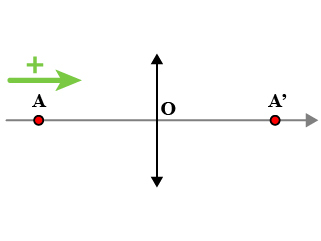
\includegraphics[max size={\textwidth}{0.9\textheight}, center, keepaspectratio]{QCM/Physique/UTC-002/lentille.jpg}
\end{minipage}
}
%%%%%%%%%%%%%%% ÉNONCÉ %%%%%%%%%%%%%%%%
\vspace*{\stretch{1}}
%%%%%%%%%%%%%%% RÉPONSE %%%%%%%%%%%%%%%%
\vspace{\reponsevspace}
\begin{tikzpicture}[remember picture, overlay]
    \node [align=left, opacity=1] at ([xshift=-1.75cm, yshift=2.5cm]current page.center) {
                \color{uniscielgrey}
                \textsf{\textit{Réponses}}
            };
    \node [align=left, opacity=1] at ([xshift=1.75cm, yshift=2.5cm]current page.center) {
                \color{uniscielgrey}
                $1:\boxtimes\qquad2:\square\qquad3:\square\qquad4:\square\qquad$\\
                \color{uniscielgrey}
                $5:\square\qquad6:\square\qquad$
            };
\end{tikzpicture}
Attention, ici on utilise les mesures algébriques, dont le signe dépend du point initial (ici $O$) et du point final ($A$ ou $A'$). Ici le sens allant de la gauche vers la droite est pris comme positif.


%%%%%%%%%%%%%%% RÉPONSE %%%%%%%%%%%%%%%%
\vspace*{\stretch{1}}
\end{flashcard}

\cardfrontfooter{Comprendre, appliquer}{physique}
\begin{flashcard}[\cardfrontheader{Mathématiques}{L0}{Statistiques}]{
%%%%%%%%%%%%%%% ÉNONCÉ %%%%%%%%%%%%%%%%
\vspace{\enoncevspace}

\begin{minipage}[t]{0.6\linewidth}
On considère une série statistique à 13 éléments décrite par sa courbe des fréquences cumulées croissantes.

Lequel des graphiques suivant peut correspondre à son histogramme (en fréquence) ?
    \begin{enumerate}
        \item Dessin de gauche
        \item Dessin du milieu
    	\item Dessin de droite
    \end{enumerate}
\end{minipage}%
\hfill
\begin{minipage}[t]{0.3\linewidth}
    \strut\vspace*{-\baselineskip}\newline
    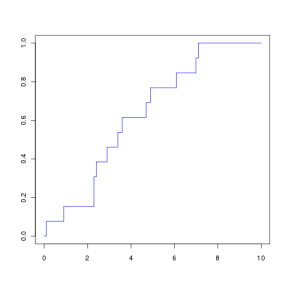
\includegraphics[max size={\textwidth}{0.5\textheight}, center, keepaspectratio]{QCM/Mathematiques/UTC-052/freq_cumulees.png}
    \includegraphics[max size={\textwidth}{0.5\textheight}, center, keepaspectratio]{QCM/Mathematiques/UTC-052/histo_fréq.png}
\end{minipage}
}
%%%%%%%%%%%%%%% ÉNONCÉ %%%%%%%%%%%%%%%%
\vspace*{\stretch{1}}
%%%%%%%%%%%%%%% RÉPONSE %%%%%%%%%%%%%%%%
\vspace{\reponsevspace}
\begin{tikzpicture}[remember picture, overlay]
    \node [align=left, opacity=1] at ([xshift=-1.75cm, yshift=2.5cm]current page.center) {
                \color{uniscielgrey}
                \textsf{\textit{Réponses}}
            };
    \node [align=left, opacity=1] at ([xshift=1.75cm, yshift=2.5cm]current page.center) {
                \color{uniscielgrey}
                $1:\boxtimes\qquad2:\square\qquad3:\square\qquad4:\square\qquad$\\
                \color{uniscielgrey}
                $5:\square\qquad6:\square\qquad$
            };
\end{tikzpicture}
D'après le graphe des fréquences cumulées, le minimum de la série est proche de 0.

Le maximum de la série associée au dessin du milieu est supérieur à 8; ce ne peut donc être la bonne réponse.

Il n'y a aucun élément entre 2 et 4 dans la série associée au diagramme de gauche; ce ne peut donc être la bonne réponse.

Le dessin de droite correspond à la série initiale.
%%%%%%%%%%%%%%% RÉPONSE %%%%%%%%%%%%%%%%
\vspace*{\stretch{1}}
\end{flashcard}

\cardfrontfooter{Changement de langage}{physique}
\begin{flashcard}[\cardfrontheader{Mathématiques}{L0}{Second degré, \'Equations/Inéquations}]{
%%%%%%%%%%%%%%% ÉNONCÉ %%%%%%%%%%%%%%%%
\vspace{\enoncevspace}
L'équation $4x^2-4x-6 = 0$ a pour  solutions dans $\mathbb R$ :
\begin{enumerate}
    \item $\displaystyle\frac{1-\sqrt7}{2}$ et $\displaystyle\frac{1+\sqrt7}{2}$.
    \item $\displaystyle\frac{-1+\sqrt7}{2}$ et $\displaystyle \frac{1+\sqrt7}{2}$.
    \item $\displaystyle\frac{-1+\sqrt7}{2}$ et $\displaystyle\frac{1-\sqrt7}{2}$.
\end{enumerate}
}
%%%%%%%%%%%%%%% ÉNONCÉ %%%%%%%%%%%%%%%%
\vspace*{\stretch{1}}
%%%%%%%%%%%%%%% RÉPONSE %%%%%%%%%%%%%%%%
\vspace{\reponsevspace}
\begin{tikzpicture}[remember picture, overlay]
    \node [align=left, opacity=1] at ([xshift=-1.75cm, yshift=2.5cm]current page.center) {
                \color{uniscielgrey}
                \textsf{\textit{Réponses}}
            };
    \node [align=left, opacity=1] at ([xshift=1.75cm, yshift=2.5cm]current page.center) {
                \color{uniscielgrey}
                $1:\boxtimes\qquad2:\square\qquad3:\square\qquad4:\square\qquad$\\
                \color{uniscielgrey}
                $5:\square\qquad6:\square\qquad$
            };
\end{tikzpicture}
On peut vérifier que $\displaystyle\frac{1-\sqrt7}{2}$ et $\displaystyle\frac{1+\sqrt7}{2}$ sont solutions. On peut aussi calculer le discriminant du trinôme on trouve $16\times 7$ et les solutions sont $\displaystyle\frac{4-4\sqrt 7 }{8}$ et $\displaystyle\frac{4+4\sqrt 7 }{8}$.

%%%%%%%%%%%%%%% RÉPONSE %%%%%%%%%%%%%%%%
\vspace*{\stretch{1}}
\end{flashcard}

\cardfrontfooter{Changement de langage}{physique}
\begin{flashcard}[\cardfrontheader{Mathématiques}{L0}{Algèbre linéaire}]{
%%%%%%%%%%%%%%% ÉNONCÉ %%%%%%%%%%%%%%%%
\vspace{\enoncevspace}
Le système   $(\cal S )\; \left\{\begin{array}{ccc} x-y+z&=&0\\ 3x +4y-z&=&0\\ -10+y-z&=&0\end{array} \right.$ a pour solution :

\begin{enumerate}
    \item $(0; 5;-5)$.
    \item $(10; \displaystyle\frac {100}{3}; \displaystyle\frac{-70}{3})$.
    \item $(10; \displaystyle\frac {100}{3}; \displaystyle \frac{70}{3})$.
\end{enumerate}
}
%%%%%%%%%%%%%%% ÉNONCÉ %%%%%%%%%%%%%%%%
\vspace*{\stretch{1}}
%%%%%%%%%%%%%%% RÉPONSE %%%%%%%%%%%%%%%%
\vspace{\reponsevspace}
\begin{tikzpicture}[remember picture, overlay]
    \node [align=left, opacity=1] at ([xshift=-1.75cm, yshift=2.5cm]current page.center) {
                \color{uniscielgrey}
                \textsf{\textit{Réponses}}
            };
    \node [align=left, opacity=1] at ([xshift=1.75cm, yshift=2.5cm]current page.center) {
                \color{uniscielgrey}
                $1:\boxtimes\qquad2:\square\qquad3:\square\qquad4:\square\qquad$\\
                \color{uniscielgrey}
                $5:\square\qquad6:\square\qquad$
            };
\end{tikzpicture}
\footnotesize
Si on réécrit le système $(\cal S )\;\left\{\begin{array}{lllc} x-y+z&=&0& \; (L_1) \\3x+4y-z&=&0& \; (L_2) \\\,\,\,\,\,\,\,\,y-z&=&10 & \; (L_3) \end{array} \right.$, qui est équivalent à $\left\{\begin{array}{llllllc} x&-y+z&=&0& \; (L_1) \\&7y-4z&=&0& \; (L_2\leftarrow L_2-3L_1) \\&y\,\,\,-z&=&10&\; (L_3) \end{array} \right.$, ou encore à $\left\{\begin{array}{llllllc} x&-y+z&=&0& \; (L_1) \\&7y-4z&=&0& \; (L_2) \\ &\;\;\,\,\,\,\,-3z&=&70 &\; (L_3\leftarrow 7L_3-L_2) \end{array} \right.$.

On a donc $z = \displaystyle \frac{-70}{3}$, $y = 10+z=10 -  \displaystyle \frac{-70}{3}= \displaystyle \frac{100}{3}$ et $x = y-z= 10$.


%%%%%%%%%%%%%%% RÉPONSE %%%%%%%%%%%%%%%%
\vspace*{\stretch{1}}
\end{flashcard}


\end{document}


